\documentclass[a4paper,14pt]{extreport}
\usepackage[left=1.5cm,right=1.5cm,
    top=1.5cm,bottom=1.5cm,bindingoffset=0cm]{geometry}
\usepackage{scrextend}
\usepackage[T1,T2A]{fontenc}
\usepackage[utf8]{inputenc}
\usepackage[english,russian,ukrainian]{babel}
\usepackage{tabularx}
\usepackage{amssymb}
\usepackage{color}
\usepackage{amsmath}
\usepackage{mathrsfs}
\usepackage{listings}
\usepackage{graphicx}
\graphicspath{ {./images/} }
\usepackage{lipsum}
\usepackage{xcolor}
\usepackage{hyperref}
\usepackage{tcolorbox}
\usepackage{tikz}
\usepackage[framemethod=TikZ]{mdframed}
\usepackage{wrapfig,boxedminipage,lipsum}
\mdfdefinestyle{MyFrame}{%
linecolor=blue,outerlinewidth=2pt,roundcorner=20pt,innertopmargin=\baselineskip,innerbottommargin=\baselineskip,innerrightmargin=20pt,innerleftmargin=20pt,backgroundcolor=gray!50!white}
 \usepackage{csvsimple}
 \usepackage{supertabular}
\usepackage{pdflscape}
\usepackage{fancyvrb}
%\usepackage{comment}
\definecolor{ggreen}{rgb}{0.4,1,0}
\definecolor{amber}{rgb}{1.0, 0.75, 0.0}
\definecolor{babyblue}{rgb}{0.54, 0.81, 0.94}
\definecolor{arylideyellow}{rgb}{0.91, 0.84, 0.42}
\usepackage{array,tabularx}
\usepackage{colortbl}

\usepackage{varwidth}
\tcbuselibrary{skins}
\usepackage{fancybox}

\usetikzlibrary{calc}
\makeatletter
\newlength{\mylength}
\xdef\CircleFactor{1.1}
\setlength\mylength{\dimexpr\f@size pt}
\newsavebox{\mybox}
\newcommand*\circled[2][draw=blue]{\savebox\mybox{\vbox{\vphantom{WL1/}#1}}\setlength\mylength{\dimexpr\CircleFactor\dimexpr\ht\mybox+\dp\mybox\relax\relax}\tikzset{mystyle/.style={circle,#1,minimum height={\mylength}}}
\tikz[baseline=(char.base)]
\node[mystyle] (char) {#2};}
\makeatother

\usepackage{float}
\usepackage{wrapfig}
\usepackage{framed}


\begin{document}
\pagecolor{white}


\begin{center}
Variant №4\\
\vspace{0.5cm}
Bohdan Lyshchenko DP-82
\end{center}

\begin{center}
4. Особливості статистики Фермі
\end{center}
\vspace{1cm}



\begin{figure}[h]
\center{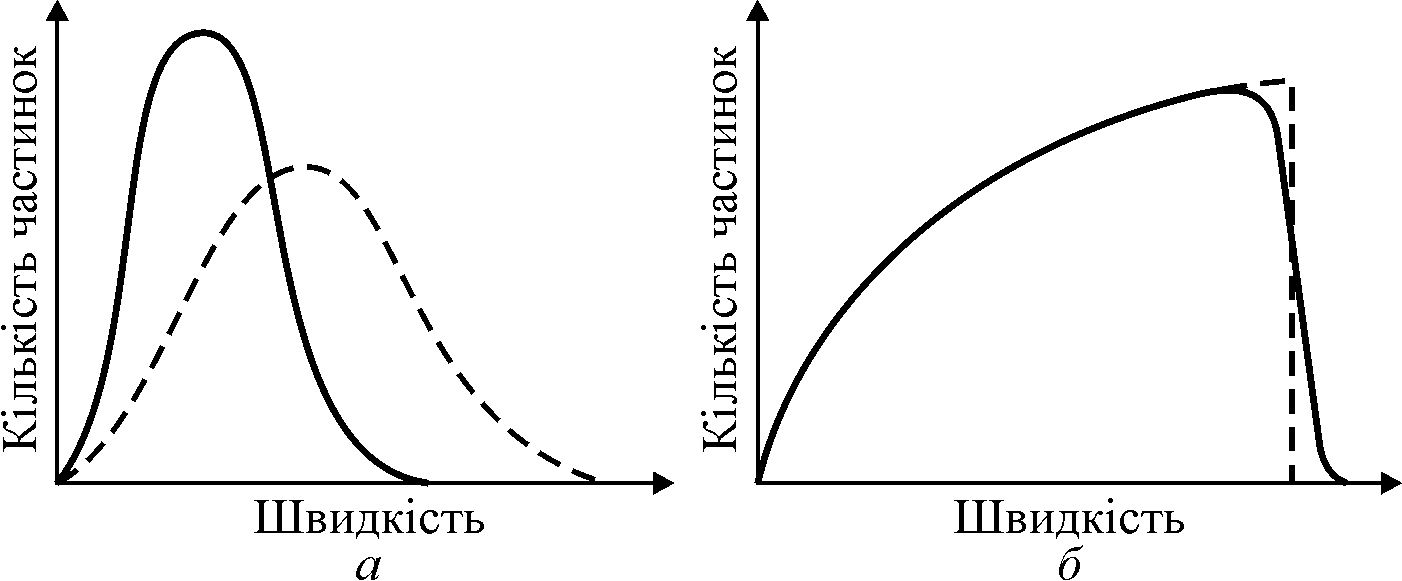
\includegraphics[width=0.5\linewidth]{1.png}}
\caption{Comparison of classical (a) and quantum (b) particle velocity distribution:
  a - distribution of gas molecules according to Maxwell-Boltzmann statistics;
b - Fermi – Dirac quantum distribution for electron gas in metal}
\label{ris1}
\end{figure}


The Fermi-Dirac statistics for an ideal gas of fermions (fermi-gas) by states with different energies is described by a distribution function:

\begin{equation}
f(E)=\left\{\exp \left[(E-\mu) / k_{B} T\right]+1\right\}^{-1}
\end{equation}

This expression is called the Fermi-Dirac distribution function. The electrochemical potential determines the change in the internal energy of a system when one particle is added to it, provided that all other quantities on which the internal energy depends are fixed.
The value $f(E)$ is equal to the average number of $<N(E)>$ fermions in a state with energy Ei. Therefore $<N (E)> = {exp [(E - \mu) / kBT] + 1} 1$. Since the probability must be a positive number, the value of the chemical potential is always less than the energy of the ground state of quasi-particles.\\

In the ground state fermions occupy the lowest energy levels possible. The imposition of the Pauli principle leads to the fact that at zero temperature, when the ground state is realized, all the lowest one-fermion levels are occupied.\\

The highest occupied level in such a state is called the Fermi level, and the distribution function looks like a "step", Fig. 1, b. If the temperature increases, there is a certain probability that the fermions of the system will have energies higher than the energy of the Fermi level. Because of this, there is a different probability from zero that the level with energy below the energy of the Fermi level becomes free and the "step" becomes slightly more gentle. At very high temperatures, the Fermi-Dirac distribution turns into the classical Maxwell-Boltzmann distribution.










\end{document}
